\section{Background on \glsfmtshort{WCA} applications}

\todo[inline]{Needs some trimming}

\begin{figure}
    \centering
    \begin{subfigure}{\columnwidth}
        \centering
        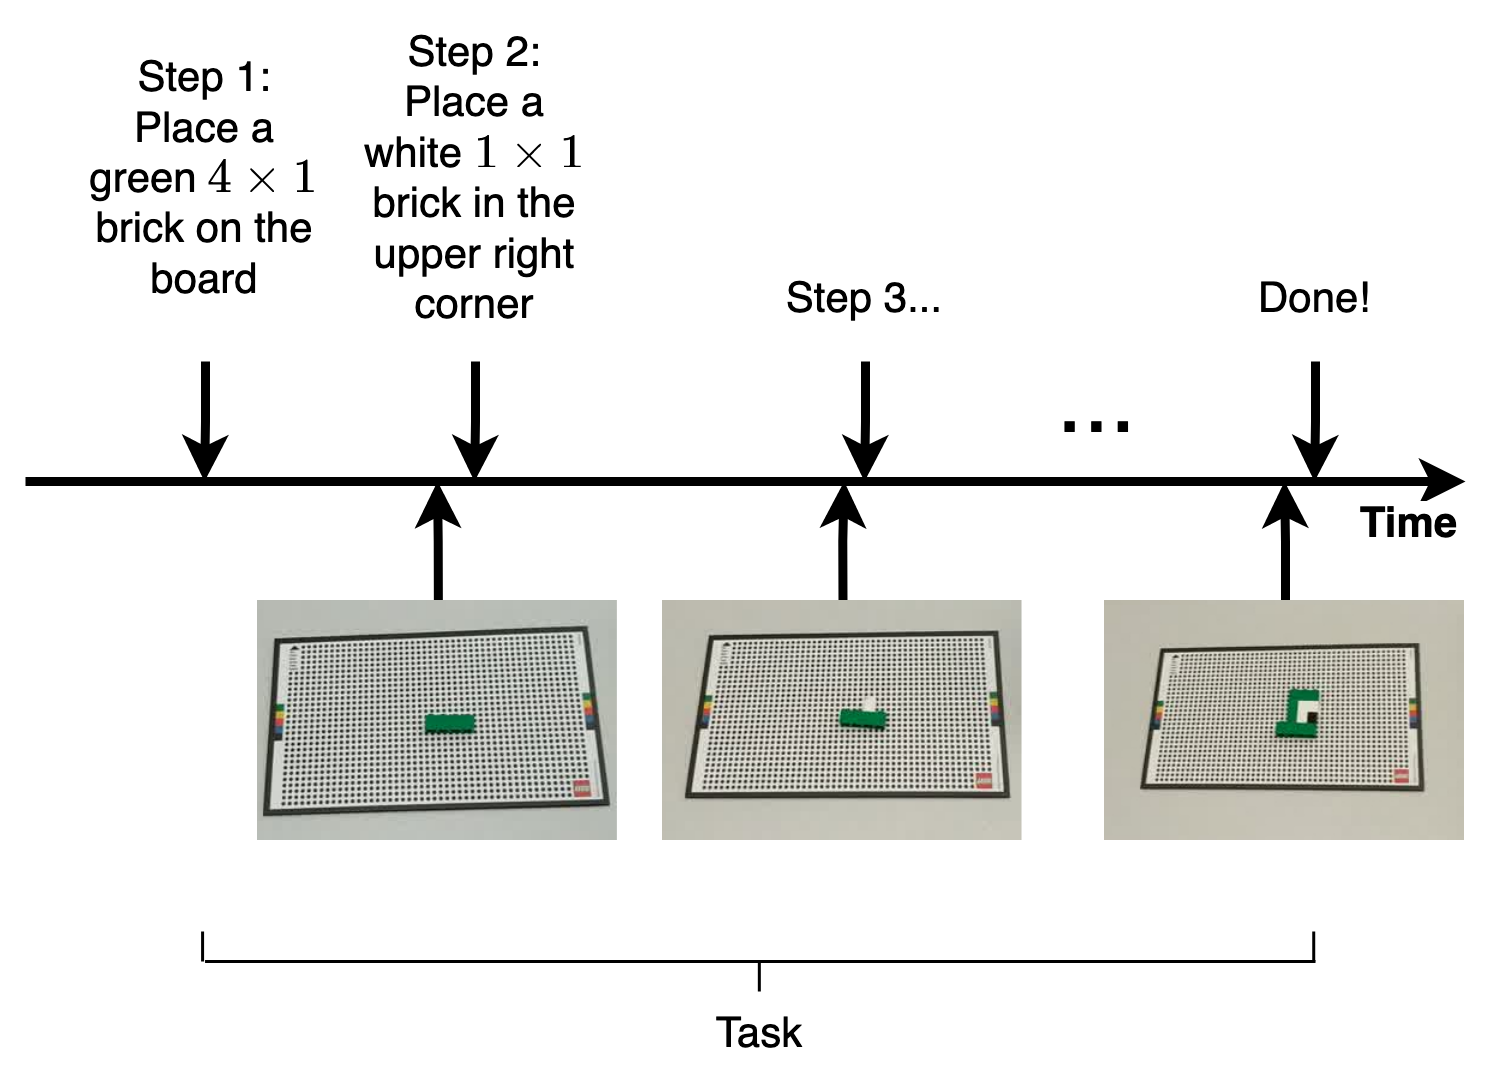
\includegraphics[width=\columnwidth]{figs/task.png}
        \caption{%
            Overview of a task in a \ac{WCA}, composed of a series of steps.
            Each steps starts with an instruction being provided to the user and ends with the instruction for the next step.
            The \ac{WCA} continuously samples the task state, automatically triggering transitions between steps as correct (or incorrect) states are recognized.
        }\label{fig:task}
    \end{subfigure}\\
    \begin{subfigure}{\columnwidth}
        \centering
        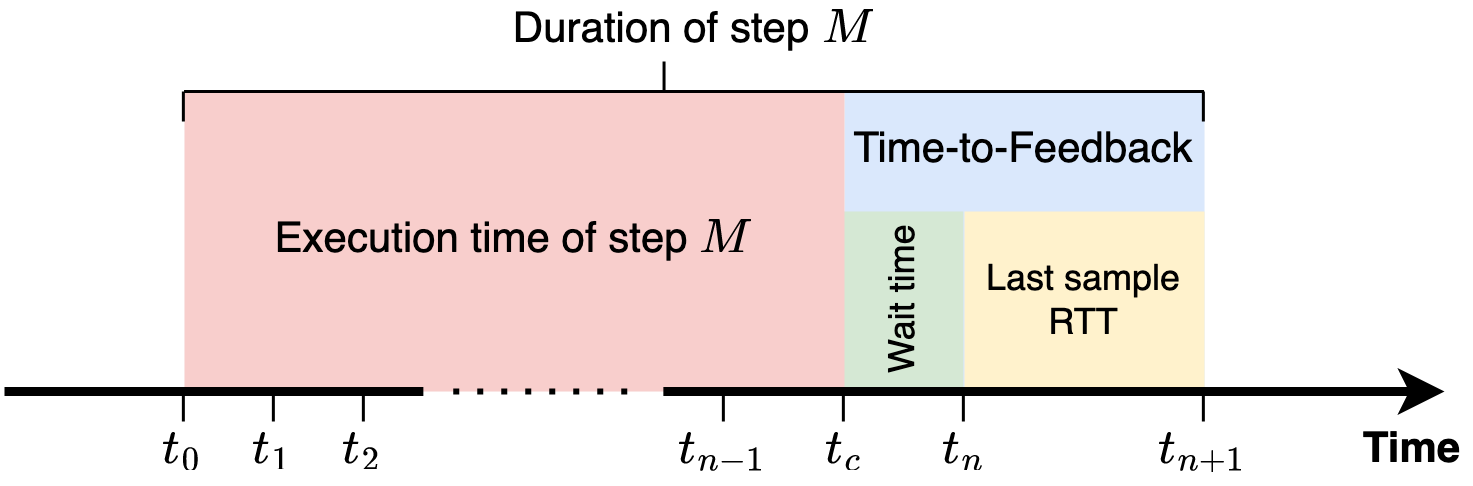
\includegraphics[width=\columnwidth]{figs/step_time.png}
        \caption{%
            Breakdown of a step into its timing components.
            The instruction for step \( M \) and \( M + 1 \) are provided to the user at \( t_0 \) and \( t_{n+1} \), respectively.
            \( t_k | k \in \{1, \ldots, n \} \) correspond to the \ac{WCA} sampling instants for step \( M \), and \( t_c \) marks the instant at which the user finishes performing the instruction.
        }\label{fig:step}
    \end{subfigure}
    \caption{Key concepts in \acl{WCA}}
\end{figure}

\acf{WCA} applications represent a category of novel, context-sensitive and highly-interactive \ac{AR} applications.
In this work we focus on a particular category --- ``step-based'' \ac{WCA} --- that have as their goal the guiding of a user through a sequential task.
Examples of such applications are the LEGO and IKEA assistants~\cite{chen2015early,chen2018application}, in which users are guided step-by-step through the process of assembling a LEGO model and an IKEA lamp, respectively.

Step-based \acp{WCA} operate analogously to how \ac{GPS} navigation assistants guide users, by seamlessly and continuously monitoring the progress of the user and autonomously providing relevant instructions and feedback.
The application follows the progress of the task in ``realtime'' by repeatedly sampling the state of the physical system, most commonly through video frames.
Whenever the assistant detects that the user has correctly or incorrectly performed an instruction, it provides a new instruction to either advance the task or correct the detected mistake.
The application otherwise remains silent and out-of-the-way of the user; that is, samples which do not generate a new instruction (e.g.~because they captured an intermediate or unfinished state, or simply noise) are silently discarded.
Herein lies one of the key characteristics of these applications: the user only consciously interacts with the application whenever they finish an instruction, and thus these are the \emph{only} points in time at which they can notice changes in system responsiveness.

In order to discuss these applications with precision we provide some definitions relating to their operation.
First of all, a \emph{step} is formally understood as a specific action to be performed by the user, described by a single instruction, and a \emph{task} consists of a series of steps to be executed in sequence (see \cref{fig:task}).
A step begins when the corresponding instruction is provided to the user, and ends when the instruction for the next step is provided; we call the time interval between these two events the \emph{step duration}.

\acp{WCA} employ sampling, most commonly of video feeds, to keep track of the state of the real world.
Take \( \{ t_0, t_1, \ldots, t_{n + 1} \} \) a series of discrete and sequential sampling instants at which the \ac{WCA} captures the state of the physical system, as illustrated in \cref{fig:step}.
\( t_0 \) corresponds to the instant at which the instruction for step \( M \) is provided and the first sample is taken, and \( t_n \) to the instant at which the final sample (i.e.\ which captures the final state of step \( M \)) is taken. 
\( t_{n + 1} \) is then the instant at which the result for sample \( t_n \) is returned and the instruction for step \( M + 1 \) is provided.
We define \( t_c \) as the point in time at which the user finishes performing the instruction for step \( M \), and the intervals \( t_c - t_0 \), \( t_n - t_c \), and \( t_{n + 1} - t_n \) as the \emph{execution time}, \emph{wait time}, and \emph{last sample \ac{RTT}}, respectively, of a step \( M \).
The sum of the latter two values (i.e.\ the interval \( t_{n + 1} - t_c \)) we call \emph{\ac{TTF}}, a metric which we will repeatedly refer to in this paper as it directly describes the responsiveness of a \ac{WCA}.

% It should be noted 
% it must follow that (see also~\cite{olguinmunoz:impact2021})\footnote{\( U(a, b) \) represents the continuous uniform distribution in the open interval \( (a, b) \).}
% % \todo[inline]{I think it's an assumption rather than a must. Specifically, it is not uniform if the general execution time distribution is Rayleigh/ExpGaussian -vishnu}
% \begin{align}\label{eq:tc}
%     t_c &\thicksim U(t_{n - 1}, t_n)
% \end{align}

% Current implementations, such as those in~\cite{Chen2015LEGO,Chen2018application}, employ \emph{greedy} sampling.
% In this scheme, a new sample is immediately taken as soon as an acknowledgement is received for the previous sample.
% This means that the interval between these sampling instants is not necessarily constant, as it is subject to fluctuations due to resource contention on both the network and compute side.
% It also has as a consequence that acknowledgements must be provided even for those samples which do not cause the generation of a new instruction --- these acknowledgements are simply used for flow control and do not generate user-noticeable feedback.